\documentclass[12pt,a4paper]{article}
\usepackage[utf8]{inputenc}
\usepackage[spanish]{babel}
\usepackage{amsmath}
\usepackage{amsfonts}
\usepackage{amssymb}
\usepackage{graphicx}
\usepackage{caption}
\usepackage{subcaption}
\graphicspath{{Imagenes/}}
\usepackage[left=2.00cm, right=2.00cm, top=2.00cm, bottom=2.00cm]{geometry}

\usepackage{float}
\setlength{\parindent}{0cm}
\setlength\parindent{0pt}

\title{Osciladores armonicos}
\author{Santiago Quintero Cordoba }
\date{}


\renewcommand{\vec}[1]{\boldsymbol{\mathrm{#1}}}


\begin{document}

\maketitle

\section*{}

Observar que aunque el sistema sea un resorte colgando podemos ignorar el efecto de la gravedad ya que ma = -(kx + mg), haciendo un cambio de sistema de coordenadas podemos llegar a la ecuación ma = -kx lo cual lo único que cambiara es la amplitud de la soluciones(sea la evolución temporal o la el espacio de fase) al igual que como se dijo anteriormente se desplazan los ejes pero el comportamiento es el mismo y las futuras conclusiones no dependen de ello, por otro lado varios libro de E.D. hacen ese cambio de coordenadas que no le ponen o quitan nada al problema a no ser que ser que se desee tener una solución exacta y no el comportamiento del sistema que tomando en cuenta nuestro sistema tampoco es que cambie mucho
\\

Lo primero que vamos a observar es como se comporta un un resorte con una masa pegada la cual parte del reposo y es elongada y por el cambio de sistema de referencia no existe termino gravitacional(de considerarse no afecta la solución homogénea y la no homogénea apenas la afecta, causando solo cambios de amplitudes y de origen), en la siguiente figura vemos la solución a dicho problema que tiene por ecuación de movimiento $\ddot{x} = - \omega^2 x$

\begin{figure}[H]
    \centering
    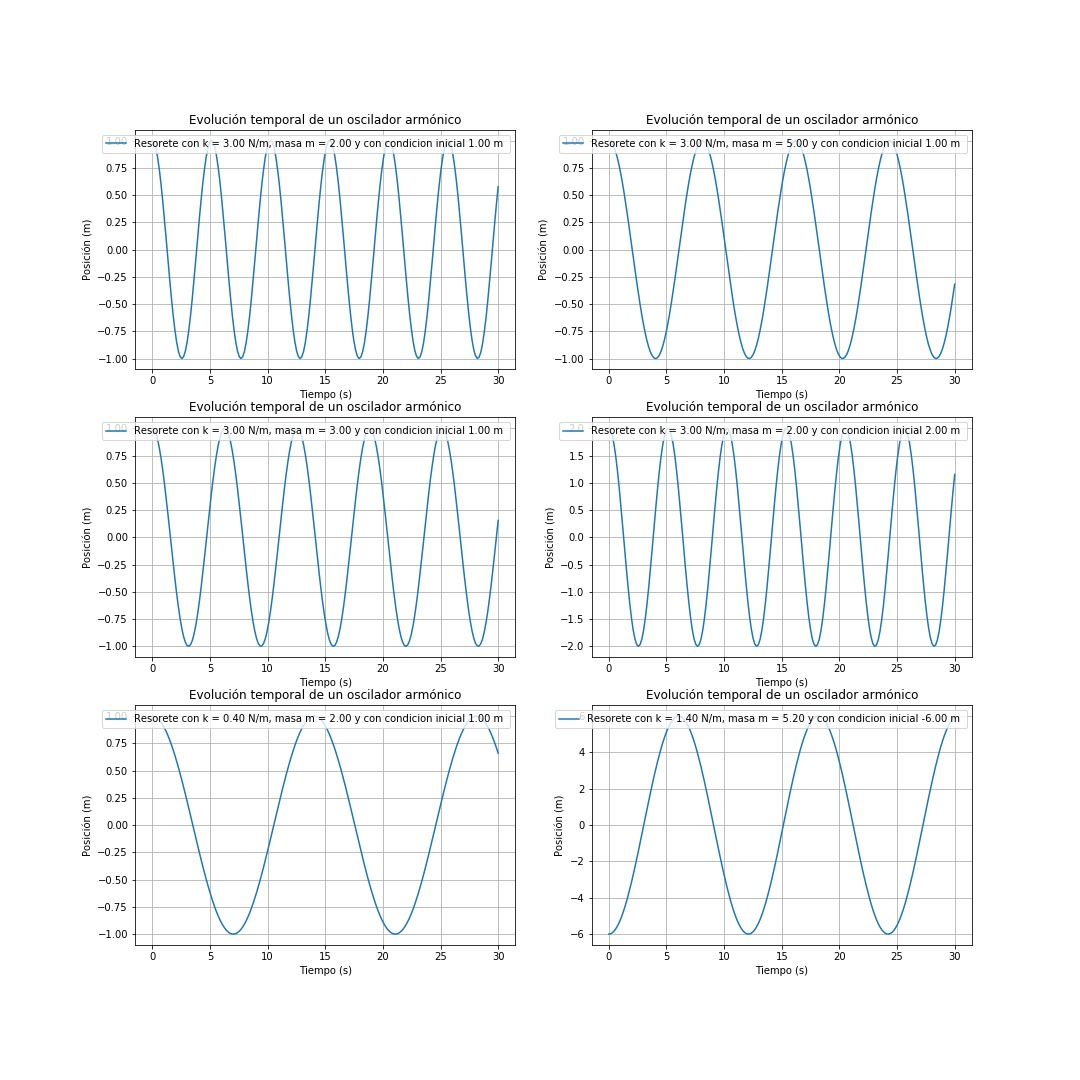
\includegraphics[width=10cm]{oscilador.jpg}
    \caption{6 osciladores armónicos diferentes}
    \label{fig:oscilador}
\end{figure}

Lo primero a observar es bajo las mismas condiciones iniciales el aumentar la masa la frecuencia del sistema aumenta(para el caso se habla de la frecuencia y no la frecuencia angular que he llamado frecuencia en el modulo), igualmente disminuir la constante elástica se aumenta la frecuencia y por otro lado la posición inicial es proporcional a la amplitud del de oscilación.
\\

Ahora observemos lo que pasa en el "espacio de fases"

\begin{figure}[H]
    \centering
    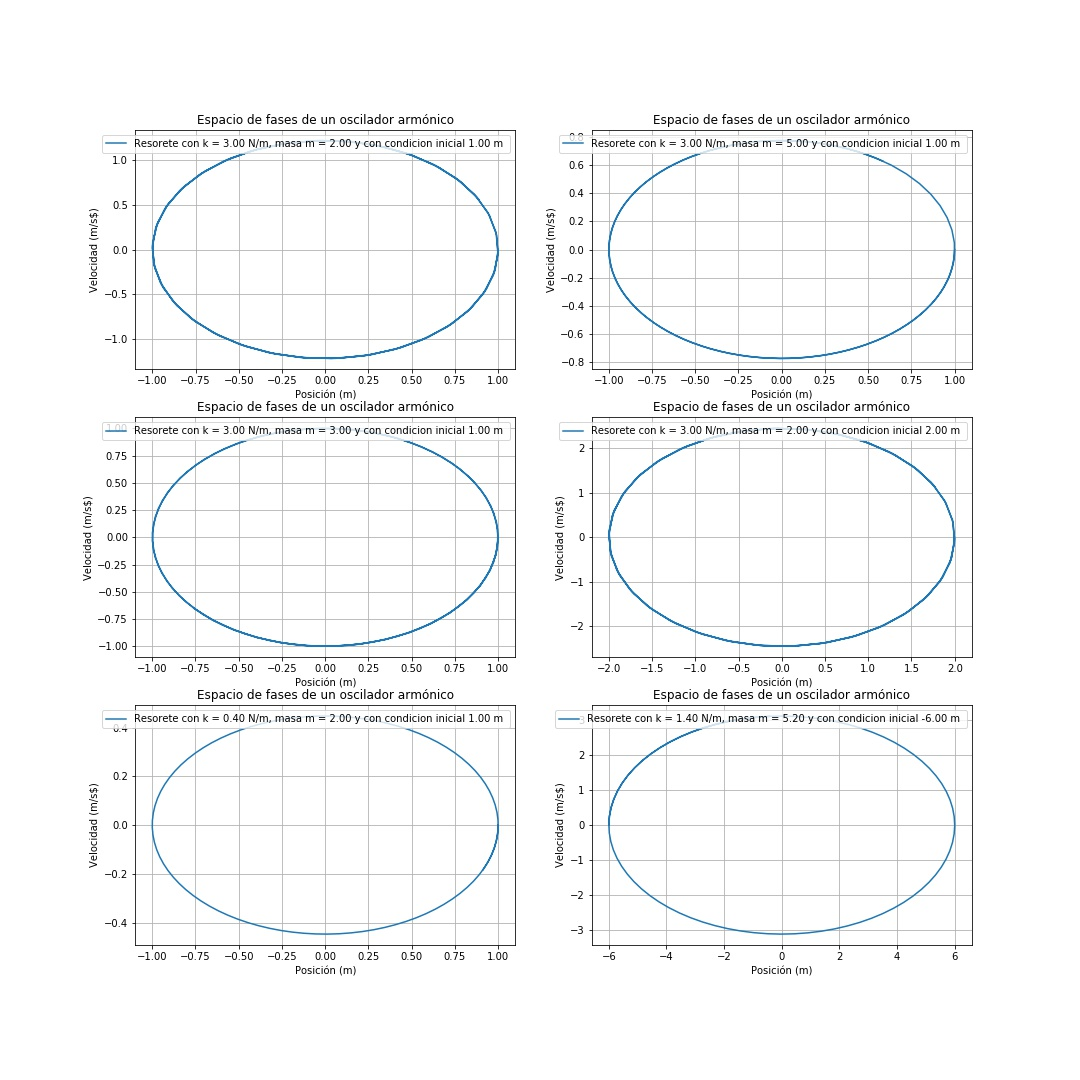
\includegraphics[width=10cm]{fases_oscilador.jpg}
    \caption{"Espacio de fases" de la figura anterior}
    \label{fig:osciladorfases}
\end{figure}

El sistema es conservativo ya que el lagrangiano no depende del tiempo, el hamiltoniano es igual a la energía y $H = E = \frac{p^2}{2m} +\omega^2 m y$ y como la energía es constante tenemos la ecuación de una elipse centrada en el origen que es lo que acabamos de hallar, es fácil ver que considerar la gravedad solo desplaza el centro de la elipse. 
\\

Ahora veamos que pasa en el sistema amortiguado, al igual que el caso amortiguado elegimos un sistema de referencia cuya solución sea independiente de efectos gravitacionales, en la siguiente figura vemos la evolución temporal del sistema cuya E.D.O es $\ddot{x} = -( - 2 \frac{2 \lambda}{m} + \omega^2 x)$

\begin{figure}[H]
    \centering
    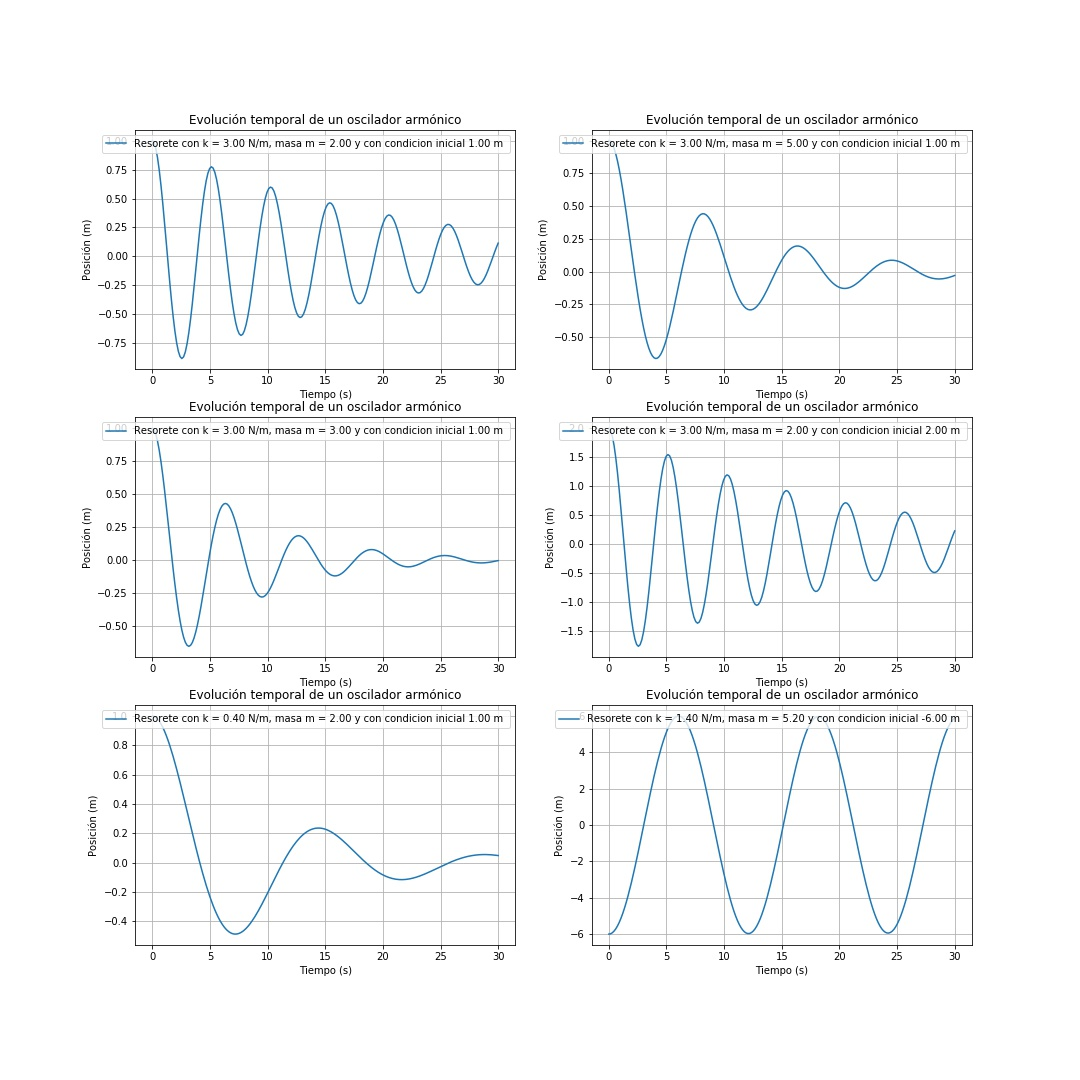
\includegraphics[width=10cm]{oscilador_amortiguado.jpg}
    \caption{6 osciladores amortiguados diferentes}
    \label{fig:oscilador_amortiguado}
\end{figure}

Como se menciona en los módulos de \cite{Landau2004} se observa que el caso interesante es cuando $\lambda << \omega$ ya que cuando es menor pero se no por mucho es caso es casi el mismo a uno sobreamortiguado(casi como el caso de la ultima figura de a lado izquierdo de figura( \ref{fig:oscilador_amortiguado})), el comportamiento es uno aperiódico(se observa que existen puntos para los cuales $y(t) \neq t(y + T)$, cuando tendemos $lambda$ a cero volvemos a tener el caso armónico.
\\

Ahora observemos el "espacio de fase" del sistema.

\begin{figure}[H]
    \centering
    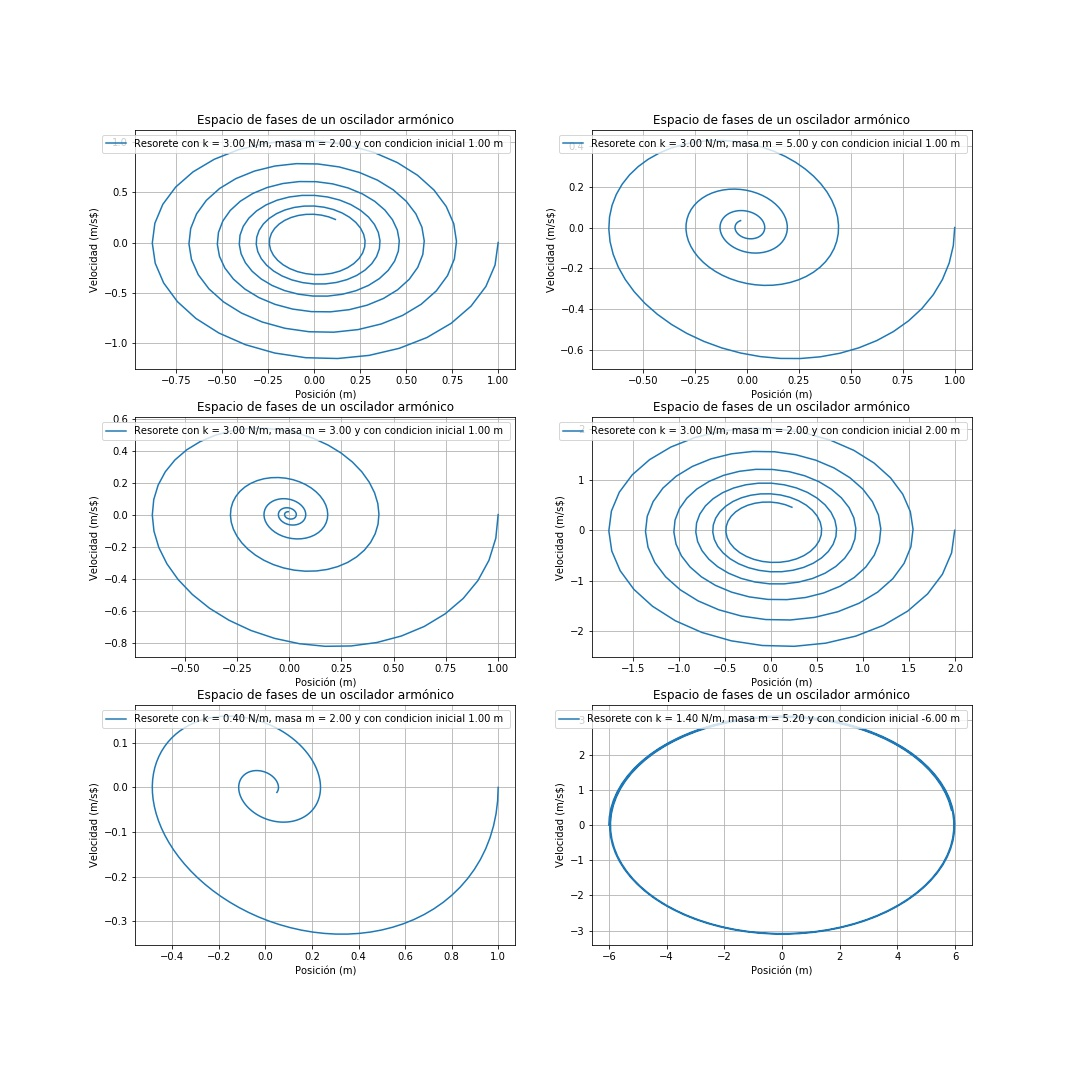
\includegraphics[width=10cm]{fases_oscilador_amortiguado.jpg}
    \caption{"Espacio de fases" de la figura anterior}
    \label{fig:osciladorfases}
\end{figure}

El hecho de que el movimiento sea aperiódico se observa en el "espacio de fase" ya que no este no es cerrado, en todos los casos vemos que el comportamiento es una espirar la cual funciona como un atractor en el origen, 

\section*{Conclusiones}

Una masa conectada a un resorte elongado el cual se cuelga se comporta como un oscilador armónico(el mismo sistema en un eje horizontal desplazado y un cambio en la amplitud) y depende tanto de la elongación inicial como de su masa y la constante del resorte y su espacio de fase muestra el comportamiento periódico del cual se observa una elipse.

En el caso del resorte en un medio el cual realiza una oposición al movimiento de tal forma que el coeficiente de amortiguamiento sea menor a la frecuencia del sistema da un movimiento aperiódico el cual tiende a cero(frenar el sistema), su espacio de fase describe una espirar cuyo inicio es un atractor. 

%===============BIBLIOGRAPHY============00
\bibliographystyle{unsrt}
\bibliography{bibliografia.bib}

\end{document}
\end{document}